\documentclass[orivec]{llncs}
\usepackage{amsfonts,amssymb,amsmath}
\usepackage{graphicx}
\usepackage{cite}
\usepackage{paralist}

\newcommand{\jMAVSim}{\textsf{jMAVSim}}

\newcommand{\naturals}{\mathbb{N}}
\newcommand{\reals}{\mathbb{R}}

\newcommand{\expectation}{\mathbb{E}}

\newcommand{\states}{S}
\newcommand{\actions}{A}
\newcommand{\observables}{O}
\newcommand{\trans}{T}
\newcommand{\obs}{Z}
\newcommand{\reward}{R}
\newcommand{\discount}{\gamma}

\newcommand{\beliefs}{\mathcal{B}}
\newcommand{\beliefUpdate}{\tau}

\newcommand{\policy}{\pi}

\newcommand{\diff}[1]{\mathop{}\!\mathrm{d}#1}

\usepackage{hyperref}

\setlength{\tabcolsep}{5pt}
% \allowdisplaybreaks

\title{Modelling and Implementation of Unmanned Aircraft Collision Avoidance}
\author{Weizhi Feng\inst{1,2},
Cheng-Chao Huang\inst{3},
Andrea Turrini\inst{1,3}\orcidID{0000-0003-4343-9323},
Yong Li\inst{1}\orcidID{0000-0002-7301-9234}
}
\institute{
State Key Laboratory of Computer Science\\Institute of Software, Chinese Academy of Sciences -- Beijing, China
\and
University of the Chinese Academy of Sciences -- Beijing, China
\and
Institute of Intelligent Software, Guangzhou -- Guangzhou, China
\email{\{fengwz,turrini,liyong\}@ios.ac.cn, huangchengchao@gziis.org}
}

\begin{document}

\maketitle

\setcounter{footnote}{0}

\begin{abstract}
	With the increasing application of unmanned aircraft in civil airspace, collision avoidance systems for unmanned aircraft are becoming more and more important and valuable.
	An ideal collision avoidance system gives the aircraft an optimal strategy for choosing flight actions to avoid collision risks when it detects other aircraft nearby.
	Currently the general approach to generating collision avoidance logics is to model the problem as a partially observable Markov decision process (POMDP), and then synthesize an optimal policy.
	However, the existing systems require the precise position information of the intruder aircraft to generate the avoidance actions and ignore the effects of the flight path changes, which may result in its lower robustness or a wasting of flying resources.

	In this paper, we construct a collision avoidance system based on limited information that reduces the variations from the original flight path.
	We use POMDPs to model the collision avoidance system with only the destination information of our own aircraft and rough information about the intruder position and generate the collision resolution logic. 
	We implement the collision avoidance module, embed it into the real unmanned aircraft system over PX4 flight control platform and demonstrate the effectiveness of our system by flight simulation.
\end{abstract}

\section{Introduction}
\label{sec:introduction}

Safety is a core requirement for aviation.
In order to increase safety, modern aviation involves pilots that are periodically trained on the airplane types they are qualified for, air-traffic controllers that instruct pilots about what route and altitude to keep and what ground movements to perform, and more and more advanced computerized control systems on board of the aircraft to help pilots to control their airplane.
One of the most dangerous situations during a flight is the possibility to have a mid-air collision.
The standard way for avoiding a collision is to implement a strict and effective air traffic control, where pilots adapt route and altitude as instructed by the air-traffic controller.
When this is not possible, e.g., in the middle of a trans-oceanic flight, pilots are assisted by aircraft on-board automation. 


\subsection{Airborne Collision Avoidance System}
\label{ssec:intro:ACAS}

As air travel became commonplace, the risk of a mid-air collision increased; 
the research on automatic aircraft collision avoidance systems gained attraction. 
In the late 1960s and early 1970s, several manufacturers developed prototype aircraft collision avoidance systems, like the Beacon Collision Avoidance System (BCAS).
BCAS uses reply data from the Air Traffic Control Radar Beacon System transponders to determine an intruder's  range and altitude.
In 1978, FAA started the development of Traffic alert and Collision Avoidance System (TCAS)~\cite{TCAS,article} widely used nowadays.
As an improvement over BCAS, TCAS can issue a resolution advisory, including a suggested ``climb'' or ``descent'' rate, to the pilot to reduce the collision risk when other aircraft are detected nearby.
After decades of development, TCAS is currently mandated on board of all large passenger and cargo aircraft worldwide.

TCAS uses an on-board beacon radar to monitor the local air traffic and logic to determine when to alert pilots to potential near mid-air collision (NMAC). 
The logic is specified using pseudocode that has been validated through simulation studies to ensure the system safety while remaining operationally acceptable. 
This decision logic was the result of decades of experience which, however, also limits its robustness.
For instance, it does not consider the scenario where pilots do not follow the suggested collision avoidance manoeuvre.
Due to the high complexity of the TCAS pseudocode, it is hard to fully understand the overall TCAS logic, let alone modify it.
See~\cite{article} for more details about TCAS and the development of airborne collision avoidance systems.


\subsection{Towards Collision Avoidance in Unmanned Aircraft}
\label{ssec:intro:toardsUAV}

In recent years, a new collision avoidance system---Airborne Collision Avoidance System X (ACAS X)~\cite{ACASX}---has been proposed and started to be investigated by many researchers.
The approach currently implemented in ACAS X is to model the aircraft nearby aviation environment as a partially observable Markov decision process (POMDP), and use dynamic programming algorithms to solve the POMDP model to get the optimal control policy ensuring as much as possible that a collision does not occur.
The collision avoidance system then stores the policy as a lookup table, queries the table and chooses the optimal action to avoid the collision when other aircraft are detected.
It has been shown in~\cite{ACASX} that ACAS X outperforms TCAS in terms of the robustness, efficiency and flexibility of the generated threat resolution logic.

ACAS Xu, the version of ACAS X specifically tailored for unmanned aircraft, is still under development. 
In fact, in recent years aviation safety needed to consider not only human-piloted airplanes, but also unmanned ones.
Unmanned aircraft are becoming more and more common in several scenarios:
from military service where they are used in several types of missions due to their lightness, hiding ability, and safety of the pilot, to civil service where unmanned aircraft can be used for aerial photography, resource exploration, express delivery, plant protection, and so on.
With the increasing number of unmanned aircraft used in public airspace, the safety of unmanned aircraft has begun to attract attention.
In particular, for mid-air collision avoidance, unmanned aircraft need to have the ability to sense other aircraft and be able to enforce the flight corrections needed to preserve the aircraft integrity.

Compared to the passenger and cargo aircraft, the design of a collision avoidance system for unmanned aircraft faces a lot of new challenges, such as more complex flying environments, weaker sensor capabilities and tight time limit to react to avoid other aircraft, which make it difficult to ensure the correctness of the collision avoidance systems for unmanned aircraft.
In particular, differently from large transport aircraft~\cite{inproceedings}, unmanned aircraft collision avoidance has to consider the following challenges: 
\begin{inparaenum}[1)]
\item
	unmanned aircraft need to sense non-cooperative traffic and tend to use cheaper, lighter, but noisier sensors due to sensor cost and payload;
\item
	aircraft flying in controlled airspace have similar performances while unmanned aircraft have a larger range of performances. 
	The resolution logic has to support more complex situations;
\item
	ACAS X only provides resolution in the vertical plane for manned aviation, but unmanned aircraft need both vertical and horizontal resolutions for safety reasons.
\end{inparaenum}

There are various previous works on collision avoidance systems for unmanned aircraft~\cite{DBLP:conf/rss/Bai-RSS-11,25,Julian-2016}.
\cite{25} modeled the collision avoidance system using POMDPs under limited observation capabilities,
applied algorithms in discrete state space to get the policy,
and performed experiments in a simulator with parameters taken from the unmanned aircraft Global Hawk.
\cite{DBLP:conf/rss/Bai-RSS-11} directly solved continuous-sate POMDPs to handle high-dimensional state space situations.
\cite{Julian-2016} used a deep neural network to learn an approximation of the lookup table.
However they do not implement the obtained avoidance logic on real flight systems, as we do in this work.
Also, their simulation results usually do not consider the impact of the generated logic on the flight path, which we also analyze.

These works are usually rather dependent on the precise detection information of the intruder aircraft (e.g. position, distance from own aircraft, etc.), as obtained from the sensors, to generate the avoidance actions.
In practice, however, due to the weak sensor capabilities and complex flying environments, it is often very difficult to obtain such a detailed information about the intruder, as well as about our own aircraft, which may result in lower robustness of the system or waste of flying resources.


\subsection{Contribution of the Paper}
\label{ssec:intro:contribution}

To address the problems described above, in this paper we construct a collision avoidance system working with limited information and minimizing the corrections to the original flight path in order to save flying resources.
We use POMDPs to model the collision avoidance system with only the destination information of our own aircraft and rough direction information of the intruder aircraft and then generate the collision resolution logic.
We evaluate the effectiveness of our proposal by implementing the collision avoidance module and running it in a Pixhawk simulator, as well as embedding it into the Pixhawk unmanned aircraft system running the PX4 flight control platform, which has been widely used for both customer drones and industrial applications, such as boats and under water vehicles.
As our experiment on flying a real Pixhawk unmanned aircraft shows (cf. Section~\ref{ssec:realDrone}), the generated avoidance logic performs well in avoiding the intruder also in real world situations.


\section{Partially Observable Markov Decision Processes}
\label{sec:MDPsandPOMDPs}

In this section we briefly recall POMDP formulation and solution methods for unmanned aircraft collision avoidance as given in~\cite{DBLP:conf/rss/Bai-RSS-11}.

Consider an agent (for example, a robot in the robotic navigation problem, or the unmanned aircraft in our setting) operating in a stochastic environment. 
The agent together with the environment represent our system, which keeps information about the state of the agent and of the environment. 
At each time step the agent, based on its view of the system state, decides what action to perform; 
this results in a change of the agent (and system) state, change that can be governed by a probability measure to model uncertainty in the outcome of the action.
When the agent has a perfect knowledge of the state of the system, it can be modeled by means of a Markov decision process~\cite{Puterman05};
when the knowledge is only partial, partially observable MDPs allow for a better modeling of the system:
in the context of unmanned aircraft equipped with noisy sensors, the exact position of an intruder is not known exactly, but only a coarse observation about its position (like: being on the left/front/right) is available.

POMDPs augment MDPs by hiding the actual states and providing an observation process that generates observations probabilistically based on the underly state. 
A POMDP models an agent decision process taking a sequence of actions to maximize the total reward obtainable from the underlying system. 
The agent, however, is not able to know precisely the underlying system state, but only gets some observations about it; 
different underlying system states can result in the same observation.
The agent keeps a belief over the system state according to the actions performed and the observations seen so far, where a belief is usually a probability measure over the system's states.


\subsection{POMDP Formulation}
\label{ssec:POMDPFormulation}

Formally, a POMDP is a 7-tuple $(\states, \actions, \observables, \trans, \obs, \reward, \discount)$ where $\states$, $\actions$, $\observables$ denote the state, action, and observation spaces of the system;
$\trans \colon \states \times \actions \times \states \to [0,1]$ and $\obs \colon \states \times \actions \times \observables \to [0,1]$ are the transition and observation functions, respectively, such that for each $s \in \states$ and $a \in \actions$, and $s' \in \states$ and $o \in \observables$, $\trans(s, a, s') = p_{\states}(s' | s, a)$ and $\obs(s, a, o) = p_{\observables}(o | s, a)$ for appropriate probability measures $p_{\states}$ and $p_{\observables}$ modelling the system's dynamics and observations, respectively; 
$\reward \colon \states \times \actions \to \reals$ is the reward function; 
and $\discount \in [0,1)$ is the discount factor balancing the trade-off between immediate and future rewards.
In the remainder of the paper, we assume that both $\actions$ and $\observables$ are finite sets.

At each step, the POMDP evolves as follows: 
when the system is in state $s \in \states$ and action $a \in \actions$ is performed, the system 
\begin{inparaenum}[1)]
\item
	gets the reward $r = \reward(s,a)$ for having performed action $a$ in $s$, 
\item
	moves to state $s'$ with probability $\trans(s, a, s')$,
\item
	and generates the observation $o \in \observables$ for $s'$ with probability $\obs(s', a, o)$.
\end{inparaenum}
Note that the observation depends on the states reached after the transition.

Since the agent has only a belief over the system state, it needs to update its belief according to the performed action $a$ and the observed observation $o$.
Let $\beliefs$ denote the set of beliefs, i.e., the set of probability measures over $\states$. 
Given $b \in \beliefs$, after taking action $a$ and observing $o$, the agent updates its belief about the system's next state $s'$ as follows:
\begin{equation} 
	b^{o}_{a}(s') = \eta \obs(s', a, o) \int_{s \in \states} \trans(s, a, s')  b(s) \diff{s},
	\label{eq:beliefUpdate}
\end{equation}
where $\eta$ is a normalization factor ensuring $\int_{s \in \states} b^{o}_{a}(s) = 1$.
To simplify the notation, we may just write $b'$ instead of $b^{o}_{a}$ when $a$ and $o$ are clear from the context.
This process of updating the belief state follows directly from Bayes' rule and is known as state estimation or filtering~\cite{book}.


\subsection{Solution Methods}
\label{ssec:POMDPSolutionMethods}

POMDPs, like MDPs, exhibit both probabilistic and nondeterministic behaviors.
The nondeterminism existing between the different actions available in a system state is resolved by a policy $\policy$ representing the agent's choice, i.e., a function $\policy \colon \beliefs \to \actions$ that specifies which action to perform based on the current belief.

The execution process of the agent alternates between action selection and belief update. 
Given $\policy$ and the agent's current belief $b$, the control of the agent takes the action $a = \policy(b)$. 
Then the belief is updated according to Eqn.~\eqref{eq:beliefUpdate}.

The goal of solving a POMDP is to synthesize an optimal policy $\policy^{*}$ maximizing the agent's expected total reward $\expectation(\sum_{n=0}^{\infty} \discount^{n} \reward(s_{n}, a_{n}))$, where $s_{n}$ and $a_{n}$ denote the system's state and chosen action at step $n$, respectively. 
A policy $\policy$ induces a value function $V_{\policy} \colon \beliefs \to \reals$ representing the expected total reward. 
The value of the total reward obtained by following $\policy$ from the belief $b$ is
\begin{equation}
	V_{\policy}(b) = \expectation\big(\sum_{n=0}^{\infty} \discount^{n} \reward(s_{n}, a_{n}) | \policy, b\big).
\end{equation}

In practice, solving POMDPs exactly is challenging due to the high computational complexity, even for relatively small-sized problems~\cite{ASurveyofPBPOMDP}. 
A variety of exact solution methods can be found in previous literature, see, e.g., the witness algorithm~\cite{article1}. 
However, these exact methods are not suitable for large-sized problems. 
To synthesize a policy for large POMDPs, approximate solution methods have been developed~\cite{article2}. 
Among them, point-based POMDP algorithms have achieved special success in computing approximate solutions to large discrete POMDPs~\cite{ASurveyofPBPOMDP,PBVI}. 
Due to the fact that the optimal value function $V^{*}$ satisfies the Bellman equation~\cite{article3}
\begin{equation}
	\begin{aligned}
		V^{*}(b) & = H(V^{*}(b)) \\
		& = \max_{a \in \actions} \Big\{\int_{s \in \states} \reward(s,a) b(s) \diff{s} + \discount \sum_{o \in \observables} p(o | b, a) V^{*}(b^{o}_{a})\Big\}
	\end{aligned}
	\label{eq:bellman}
\end{equation}
where $H$ is called the \emph{backup} operator, most of the solution methods use it to compute the optimal $V^{*}$. 
Value iteration is a commonly used dynamic programming algorithm based on the Bellman equation for solving MDP problems~\cite{RLIntro}; 
its basic structure has also been used for developing POMDP algorithms~\cite{ASurveyofPBPOMDP}. 

In the value iteration process, an initial value function $V$ is chosen so to represent the initial known information about the value;
if no information is known in advance, then $V$ is taken to be $0$ for all beliefs. 
Then it performs backup operation $H$ on $V$ by repeatedly computing the Bellman equation until the iteration process converges to a fixed point. 
Once the iteration procedure terminates, the corresponding policy is extracted by taking, for each belief $b$, the action $a$ satisfying the equality in Eqn.~\ref{eq:bellman}.

When implemented naively, the value iteration algorithm needs to search the entire belief space $\beliefs$, which will face the curse of dimensionality and exponential time complexity in large real-world-sized problems~\cite{ASurveyofPBPOMDP}. 
Two main ideas of point-based algorithms have brought about significant progress in improving computational efficiency~\cite{MCVI}. 
First, a small set of points is sampled from the belief space $\beliefs$ as an approximate representation of $\beliefs$. 
The algorithm performs backup operations over the sampled belief points rather than the entire belief space $\beliefs$ to compute the approximately optimal value function. 
Second, the $\alpha$-vectors~\cite{sarsop} are used to approximate the value function $V_{\policy} \colon \beliefs \to \reals$ representing the expected total reward of executing policy $\policy$ starting from $b$.
The optimal value function can be arbitrarily closely approximated by a piece-wise linear and convex function~\cite{Sondik78} of the form 
$
	V^{*}(b) = \max_{\alpha \in \Gamma} \alpha \cdot b
$,
where $\Gamma = \{\alpha_{0}, \alpha_{1}, \dotsc, \alpha_{m}\}$ is a set of $m$ vectors called $\alpha$-vectors.
Intuitively, each $\alpha$-vector can be associated with an action and for the current belief, the solution policy selects the action corresponding to the best $\alpha$-vector.
Thus the policy can be represented by the set $\Gamma$ of $\alpha$-vectors~\cite{sarsop}.
By using $\alpha$-vectors, we can use partial policies calculated at one belief point for other parts of the belief space $\beliefs$ under appropriate conditions, thereby significantly improving the computational efficiency~\cite{ASurveyofPBPOMDP}.

Point-based algorithms differ in how they sample the belief space and perform backup operations. 
PBVI~\cite{PBVI} has been the first point-based algorithm to work well on large POMDPs. 
HSVI2~\cite{PBVII} uses heuristics to guide sampling from the belief space, which can reduce the gap between the upper and lower bounds of the optimal value function, thus speeding up convergence. 
SARSOP~\cite{sarsop} is related to HSVI2, but it attempts to sample the optimally reachable space $\mathcal{R}^{*}(b_{0})$ from the initial belief $b_{0}$ through learning-enhanced exploration and bounding techniques.

Though point-based algorithms have made great progress in solving discrete POMDPs, progress on continuous state space POMDPs is rather limited. 
Continuous POMDP models have more powerful representation capabilities for real-world systems; 
however, they make it hard to deal with the ``curse of dimensionality''. 
One common way is to place a regular grid over $\states$ and construct a discrete POMDP model first. 
Then one can solve the latter by using existing discrete POMDP algorithms. 
The difficulty with this approach is that the discretization of the state space often results in a number of states that is still too large. 
One idea to avoid this is to use a particular parametric form to represent beliefs and value functions of states, e.g., a linear combination of Gaussian distributions~\cite{pbvic}. 
Another idea is to use particle filters to represent beliefs, like in MC-POMDP~\cite{mcpomdp}. 
MCVI (Monte Carlo Value Iteration)~\cite{MCVI} combines the method of particle-based belief representation and the key idea of discrete point-based POMDP algorithms: 
the $\alpha$-vectors. 
MCVI represents the solution policy by means of a policy graph $G$~\cite{MCVI}, that is, a directed graph that encodes the optimal policy by labeling each node of the graph with an action and each edge with an observation;
beliefs are not stored explicitly in the graph.
Given a belief $b$, MCVI synthesizes the policy from a policy graph by starting from some appropriate node $v$ of $G$. 
The action chosen by the policy is the one labeling $v$;
then the agent receives an observation $o$ and moves to the successor node $v'$ by following the edge $(v,v')$ labeled by $o$. 
This process is repeated to get the policy.

For each node $v$ of the policy graph $G$, we can define the $\alpha$-function $\alpha_{v}$: 
$\alpha_{v}(s)$ is the expected total reward of executing $\policy_{G,v}$ from the current state $s$:
\begin{equation}
\label{eq:alphaPolicy}
	\alpha_{v}(s) = \expectation\big(\sum_{n=0}^{\infty} \discount^{n} \reward(s_{n}, a_{n}) | \policy_{G,v}, s\big).
\end{equation}
Then the value of $b$ with $\policy_{G,v}$ is defined by the $\alpha$-functions associated with $G$:
\begin{equation}
	V_{G}(b) = \max_{v \in G} \int_{s\in S} \alpha_{v}(s) b(s) \diff{s}.
\end{equation}

The policy graph is constructed by approximate dynamic programming techniques and MCVI performs Monte Carlo (MC) simulation to sample the state space and the corresponding belief space. 
The optimal POMDP value function $V^{*}$ is computed iteratively according to the backup operation in Eqn.~\eqref{eq:bellman}, i.e., by the Bellman equation, on each belief $b$ in the reachable belief set. 
Each backup can choose an action that maximizes the sum of the expected immediate reward and the expected total reward at the next belief. 
Then the action is added to the policy graph to make it closer to the optimal policy. 
The reachable belief set is sampled from the whole belief space as an approximate representation of the belief space. 
The MCVI method performs well in dealing with integral calculations in continuous state problems, thus avoiding to discretize the state space as a grid and improving its efficiency. 
For more details, see~\cite{MCVI}.


\section{Collision Avoidance Models}
\label{sec:collisionAvoidanceModels}

To the best of our knowledge, the algorithms and models used in the latest versions of ACAS X and ACAS Xu are not publicly accessible.
Therefore, we define our model based on the early published version of ACAS X~\cite{ACASX} and ACAS Xu~\cite{DBLP:conf/rss/Bai-RSS-11}.
In our implementation, the aircraft model is parametric and can be easily modified to fit different types of aircraft.
In this work, we use the parameter values from Pixhawk\footnote{\url{https://pixhawk.org/}} and build the model with PX4\footnote{\url{https://dev.px4.io/master/en/index.html}, PX4 Development Guide.}. 

In our model, we consider a simple encounter situation between two aircraft, our own aircraft and an intruder aircraft.
Our own aircraft has no prior knowledge about the flight path of the intruder aircraft, when an encounter happens.
During this period, our own aircraft can only get information about the intruder aircraft's elevation and bearing by sensors onboard.
The collision avoidance system is responsible to control our own aircraft so to keep a safe distance from the intruder by choosing appropriate actions to avoid collision. 

We will describe the state-transition, observation and reward modeling in our model in detail, similarly to the modeling proposed in~\cite{DBLP:conf/rss/Bai-RSS-11}.


\subsection{State-Transition Modeling}
\label{ssec:stateTransitionModeling}

\begin{figure}[t] 
	\centering
	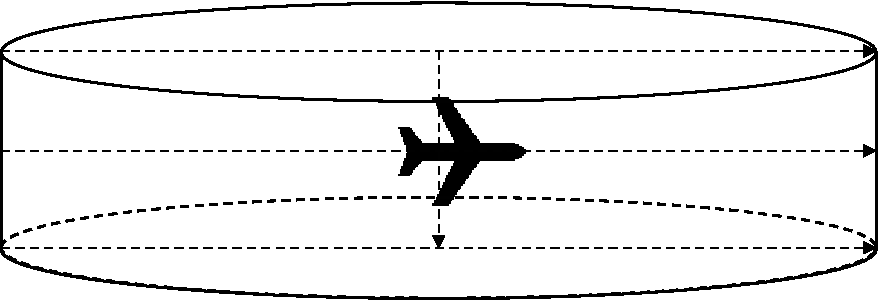
\includegraphics[width=0.40\linewidth]{3dsystem}
	\caption{Threshold range for starting the system in 3D}
	\label{fig:3dsystem}
\end{figure}
The position of a flying aircraft can be represented as a point in the 3-dimensional space.
The collision avoidance system needs to intervene when the horizontal and vertical distances of two aircraft are less than the given thresholds, which depend on the type of the aircraft and other parameters; 
this can be represented as the cylinder shown in Fig.~\ref{fig:3dsystem}.

Similarly to other works on collision avoidance~\cite{25,ACASX}, in order to simplify the model's state space and make verification more practical, we omit the altitude and consider only the latitude/longitude of the aircraft.
So when an intruder is detected, the system tries to avoid the collision by banking left or right, i.e., by changing our aircraft's direction.


\subsubsection{State space.}
Since we ignore the aircraft altitude in our model, we let $(x, y)$ be the position of the aircraft with respect to the Earth coordinate system, where the positive $x$-direction points East and the positive $y$-direction points North.
Let $\theta$ be the heading angle of the aircraft with respect to East and $u$ the aircraft's horizontal forward speed.
The state information of each aircraft is then $(x, y, \theta, u)$.
By combining the information about our aircraft and the intruder, a state in the POMDP representing our model is a $7$-tuple $(x_{1}, y_{1}, \theta_{1}, x_{2}, y_{2}, \theta_{2}, u)$, where $(x_{1}, y_{1}, \theta_{1}, u)$ stands for the state of our own aircraft while $(x_{2}, y_{2}, \theta_{2}, u)$ is the intruder's state, by assuming that both aircraft have the same speed.

The state space of the POMDP is continuous, given the nature of the aircraft information.
In order to compute the next action for our own aircraft, traditional methods have to first discretize the state space by means of a grid, where each grid cell becomes a state of the discrete POMDP~\cite{article}.
In our model, we will directly work in the continuous state space instead.
In this way, we can apply Monte Carlo methods to improve efficiency of the computation of the policy. 

\subsubsection{Action space.}
Now we introduce our modeling of actions.
In order to avoid a collision in an encounter situation, we can change our aircraft direction by changing its forward angle, that is, we bank the aircraft.
Thus we can represent the angular velocity $\omega \in \{-\omega_{m}, 0, \omega_{m}\}$ as an action in our model, where $\omega_{m}$ is the maximum input value for the banking rate.
Consequently, if at step $t$ the heading angle is $\theta_{t}$ and we take the action $\omega$, then the heading angle will become $\theta_{t+1} = \theta_{t} + \omega \Delta t$ at step $t+1 = t + \Delta t$ after a small duration of time $\Delta t$.

\subsubsection{Transition dynamics.}
Now we are ready to give the state-transition dynamics of an aircraft in an encounter situation.
Recall that in our model, a state consists of the information about both aircraft.
Let $s_{t}$ be the state at step $t$ and $s_{t+1}$ the new state at step $t+1$ after a small duration of time $\Delta t$, where $\Delta t$ is the sum of two small durations $\Delta t_{h}$ and $\Delta t_{f}$, i.e., $\Delta t = \Delta t_{h} + \Delta t_{f}$.
In order to avoid a collision, our own aircraft first changes the heading angle by banking $\omega$ degrees for a small amount of time $\Delta t_{h}$ and then goes forward at the constant speed $u$.
After a small amount of time $\Delta t_{u}$, our own aircraft will reach the new position $(x_{t+1}, y_{t+1})$ from $(x_{t},y_{t})$.
This transition dynamics is formalized as follows.
\begin{equation} 
\label{eq:transition}
	\begin{split}
		\theta_{t+1} &= \theta_{t} + \omega \Delta t_{h},\\
		x_{t+1} &= x_{t} + u \Delta t_{f} \cos \theta_{t+1},\\
		y_{t+1} &= y_{t} + u \Delta t_{f} \sin \theta_{t+1}.
	\end{split}
\end{equation}

Note that at the same time, the intruder will also change its flight state $(x_{2}, y_{2}, \theta_{2}, u)$ in a similar way by following the action $\omega_{\mathit{intruder}}$.
Since our own aircraft does not know the action of the intruder, we can model it in different ways:
for instance, the action $\omega_{\mathit{intruder}}$ can be chosen between bank-left, go-forward, and bank-right with equal probability of $\frac{1}{3}$.
Other policies can be used to represent different flight plans for the intruder, such as always banking left or right, to represent an intruder flying in circle;
we can also consider policies where the intruder tries to intercept our aircraft.
We leave the analysis of such policies to the extended version of this paper.



\subsection{Sensor Modeling}
\label{ssec:sensorModeling}

\begin{figure}[t]
	\centering
	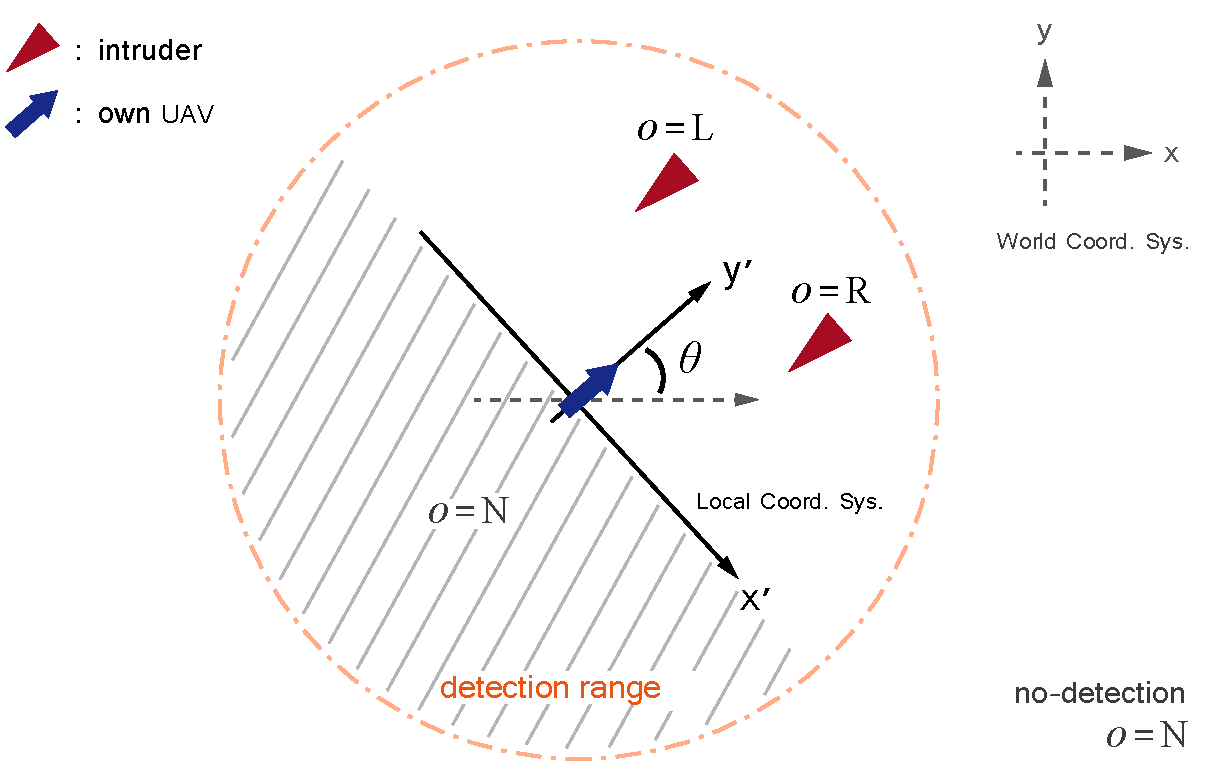
\includegraphics[width=0.7\linewidth]{observationModel}
	\caption{Observation Model}
	\label{fig:observationModel}
\end{figure}
The threat resolution logic behind a collision avoidance system relies on the aircraft on-board sensors to detect intruders.
Electro-optical/infrared (EO/IR) sensors and passive radars are two types of sensors commonly used on large aircraft.
On smaller aircraft, the on-board sensors usually have limited accuracy;
to model this scenario, we use as possible observations $\{N, L, R\}$, which stand for the fact that no intruder is detected, it is detected on the left of the aircraft, or on the right, respectively. 
Fig.~\ref{fig:observationModel} shows the observation values corresponding to the possible positions of the intruder with respect to our own aircraft.


By following the state modeling introduced in Section~\ref{ssec:stateTransitionModeling}, we can let $(x_{1},y_{1})$ be the coordinates of our aircraft in the Earth coordinate system and $\theta$ its heading angle with respect to East.
Let $(x_{2},y_{2})$ be the coordinates of the intruder in the Earth coordinate system and $(x'_{2},y'_{2})$ be the corresponding coordinates in the local coordinate system of our own aircraft, which is represented in Fig.~\ref{fig:observationModel} by the $x'y'$-coordinate system whose origin coincides with our aircraft.
In order to get the position of the intruder with respect to our own aircraft, we convert the coordinates of the intruder into our local coordinate system as follows:
\begin{equation}
\label{eq:convert}
\begin{split}
    x'_{2} &= (x_{2}-x_{1}) \sin\theta - (y_{2}-y_{1}) \cos\theta,  \\
    y'_{2} &= (x_{2}-x_{1}) \cos\theta + (y_{2}-y_{1}) \sin\theta.
\end{split}
\end{equation}
We let $d$ denote the horizontal relative distance of two aircraft and $o$ denote the observation value of the intruder;
the value $d$ can be computed as
\begin{equation}
	\label{eq:distance}
    d = \sqrt{(x_{1}-x_{2})^{2} + (y_{1}-y_{2})^{2}} = \sqrt{{x'_{2}}^{2} + {y'_{2}}^{2}},
\end{equation}
while the value for $o$, for a given detection range $r$, is
\begin{equation} 
	o = 
	\begin{cases}
		N & \text{if $y'_{2} < 0 \lor d > r$,} \\
		L & \text{if $y'_{2} \geq 0 \land d \leq r \land x'_{2} < 0$, and} \\
		R & \text{if $y'_{2} \geq 0 \land d \leq r \land x'_{2} \geq 0$.}
	\end{cases}
\end{equation}


\subsection{Reward Modeling}
\label{ssec:rewardModeling}

As we have seen in Section~\ref{ssec:POMDPSolutionMethods}, a solution for a POMDP is a policy that maximizes the expected total reward.
In order to synthesize a policy piloting our own aircraft to its destination while avoiding collisions, we use rewards to compute a policy that fulfills our requirements.

When at state $s$ and the policy chooses to take action $a$, a penalty value (i.e., a negative value) $r = \reward(s, a)$ is computed:
it depends on the distance between our aircraft and the intruder, as well as the chosen action.

\begin{table}[t]
	\caption{Aircraft action rewards}
	\label{tab:NMACpenalties}
	\centering
	\begin{tabular}{c|c}
		condition on distance $d$ and banking angle $\omega$ & reward value \\
		\hline
		$d \leq \text{NMAC}$ & -100 \\
		$d > \text{NMAC}$, $\omega \neq 0$ & -1 \\
		$d > \text{NMAC}$, $\omega = 0$ & 0 \\
		$d > \text{NMAC}$, at destination & 100 
	\end{tabular}
\end{table}

Since we only consider the 2-D space, we use NMAC to represent the minimum horizontal distance between the two aircraft so that they are considered to be near collision. 
We give the large penalty of $-100$ to each action performed when the two aircraft are closer than the NMAC distance, as shown in Table~\ref{tab:NMACpenalties}.
When the aircraft are enough far away, we give a penalty of $-1$ when the action $\omega$ of our own aircraft is not zero, i.e., the aircraft changes direction, and of $0$ if it goes straight.
This allows us to reduce non-necessary actions taken by our own aircraft. 
Finally, when our aircraft reaches its destination, a reward of $100$ is given to each action, as long as the intruder is not closer than NMAC.

Regarding the discount factor for the expected reward (cf. Eqns.~\eqref{eq:bellman} and~\eqref{eq:alphaPolicy}), we use $\discount = 0.95$ as discount factor.
This values ensures that it is better to immediately avoid the intruder than eventually reach the destination; 
however, reaching the destination is still taken into account rather strongly (cf.~\cite{RLIntro}).


\section{Experimental Evaluation}
\label{sec:experiments}

We based our experiments on the implementation of MCVI~\cite{DBLP:conf/rss/Bai-RSS-11} publicly available in \url{https://github.com/bhy/mcvi}: 
it takes as input a POMDP model (coded in C++) and produces as output a policy graph file. 
We have created our own POMDP model of the collision avoidance problem by extending functions of the MCVI source code and generated the corresponding collision avoidance policy graph. 
We then extended the PX4 flight stack by adding a collision avoidance module implementing the policy synthesized by MCVI.
The performance of the collision avoidance module has then been evaluated on two scenarios.

\begin{figure}[t]
	\centering
	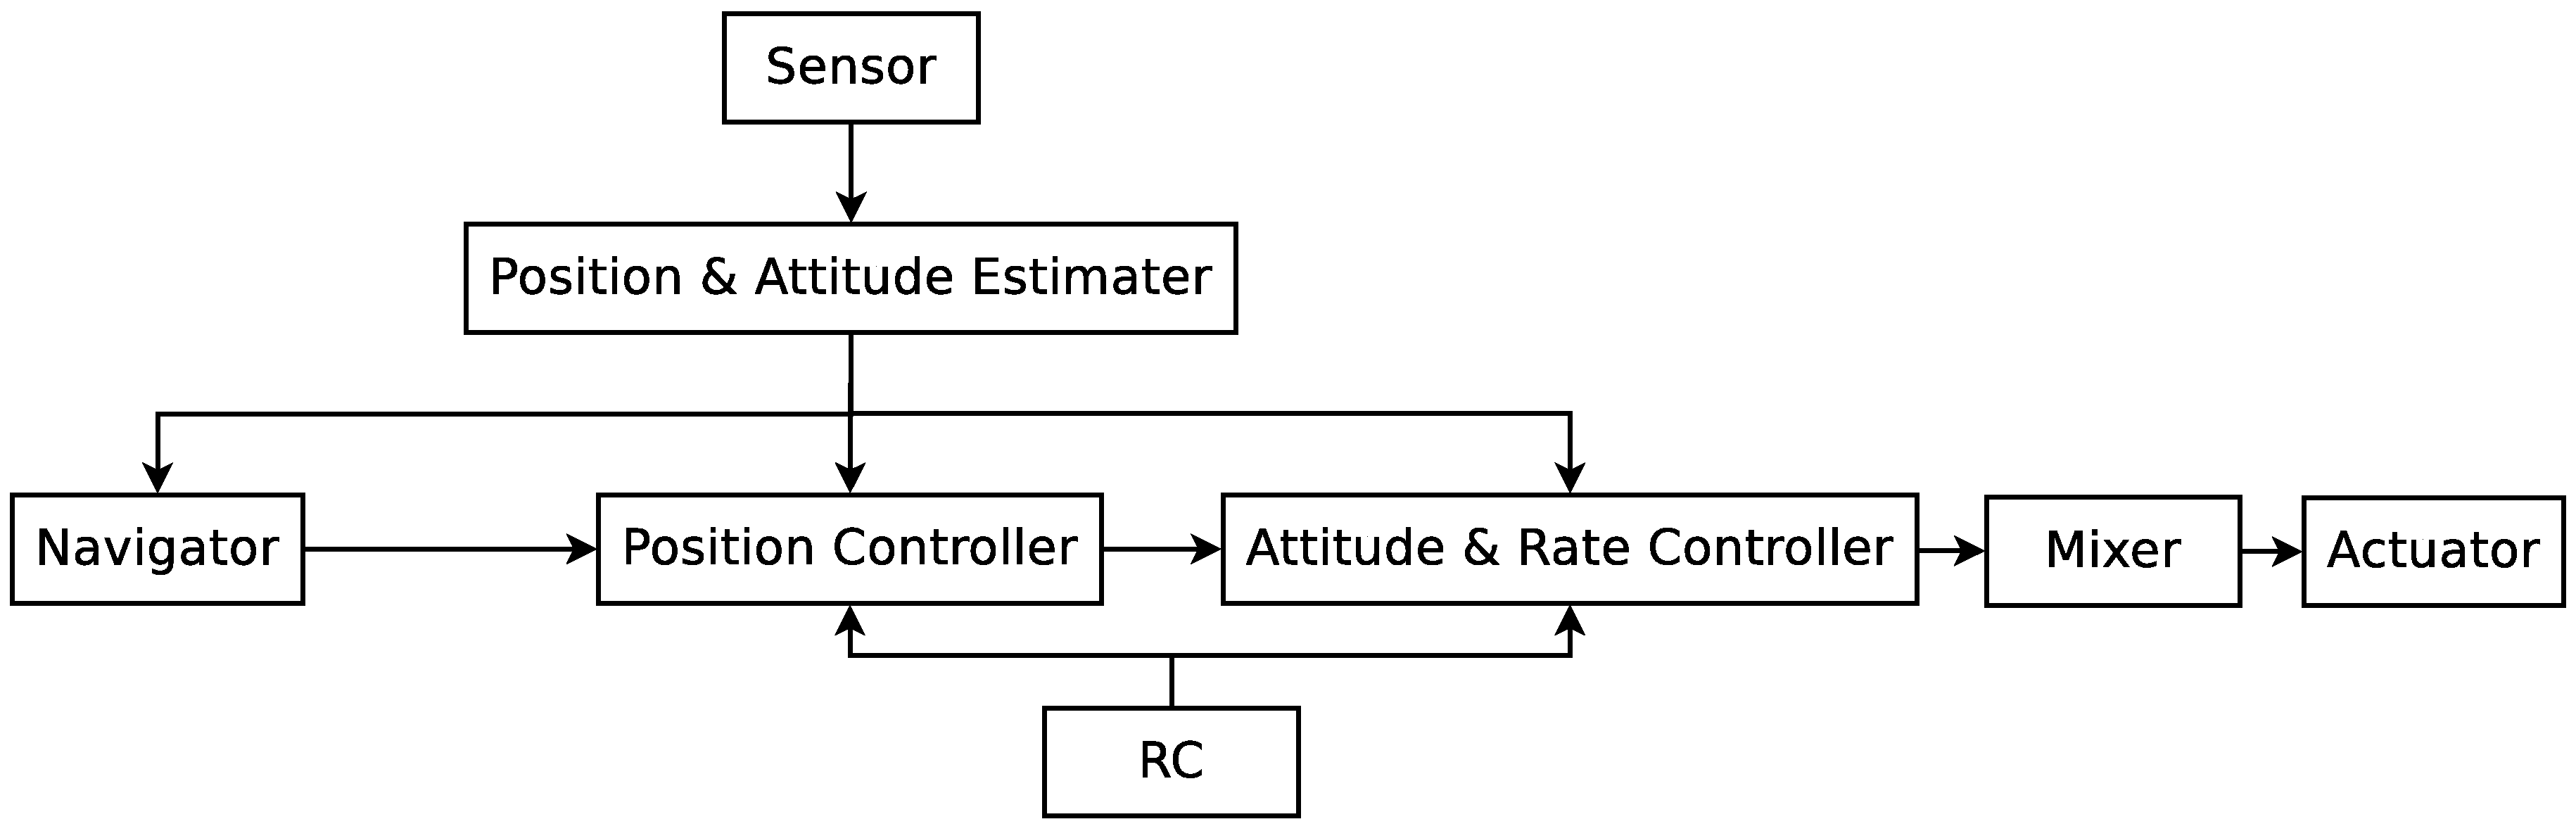
\includegraphics[width=0.9\linewidth]{flightStack.pdf}
	\caption{Overview of the PX4 flight stack}
	\label{fig:flightStack}
\end{figure}

PX4 is an open source flight control platform that is supported by the Pixhawk flight control board, an independent open-hardware project for drones and other unmanned vehicles developed by Computer Vision and Geometry Laboratory at ETH Zurich.
Due to the clear structure of PX4 flight stack, shown in Fig.~\ref{fig:flightStack}. it is easy for developers to add their own flight mode on Pixhawk hardware board with PX4 software, or in the \jMAVSim{} tool that is a simulator for PX4-controlled unmanned aircraft.
We integrated the collision avoidance module we developed into the PX4 flight stack by adding it in the  position controller, the PX4 component responsible for the flight trajectory.


\subsection{Experiments Configuration}
\label{ssec:experimentsConfiguration}

In the experiments, since our Pixhawk drone has no sensors for detecting an intruder, we have created synthetic encounter situations where our own aircraft detects an intruder while performing a flight mission, so there may be a collision. 
The flight mission of our own aircraft is to reach the destination placed at 30 meters North of the initial position. 
The intruder aircraft starts from our destination and its goal is to reach our initial position.
When an encounter occurs, the intruder aircraft is designed to fly according to two predefined policies, introduced later in Sections~\ref{ssec:oppositeFlight} and~\ref{ssec:randomInterferingFlight}.
By following the sensor modeling given in Section~\ref{ssec:sensorModeling}, our own aircraft makes a detection every second, and the detection radius is set to 10 meters. 
That is, our own aircraft gets one observation per second about the presence and position of an intruder aircraft; 
it can be sensed when the distance between the two aircraft is below 10 meters. 
After getting the observation about the intruder aircraft, our own aircraft will react according to the two different collision avoidance methods introduced below.

\paragraph*{Simple rule-based collision avoidance scenario.}
In the simple rule-based collision avoidance scenario, our own aircraft reacts to observations as follows:
if $L$ or $R$ is observed (i.e., the intruder aircraft is in the detection range on the left or right of our aircraft), then bank to the opposite direction by $\frac{\pi}{6}$ and fly forward by $1$ meter;
otherwise $N$ is observed, so fly towards to destination.

\paragraph*{MCVI-based collision avoidance scenario.}
In the collision avoidance scenario using the MCVI synthesized policy, our own aircraft reacts to observations as follows:
as soon as an intruder aircraft is detected (observations $L$ and $R$), bank according to the policy as long as the intruder is detected or the graph terminal node is reached.
If the intruder aircraft is not detected or the policy graph terminal node is reached, fly towards the destination.
The banking angle and step length are the same as those of the simple rule-based method.
Note that after the controller stops to follow the policy, if the intruder aircraft is detected again, the controller restarts to follow the policy. 

\paragraph*{Experiments setting.}
Finally, we implemented the above two collision avoidance methods in the PX4 platform.
Supported by the \textsf{Software In the Loop} (SITL) simulation of the PX4 platform, we used \jMAVSim to  simulate our experiments. 
\jMAVSim{} supports the multirotor simulation and allows us to fly drones running PX4 in a synthetic world. 
To compare the effectiveness of two collision avoidance methods, we recorded the following measure data (with the meter as the length unit) to indicate the performance:
the number \emph{actNum} of banking performed to reach the destination,
the minimum distance \emph{minDis} between our own aircraft and the intruder aircraft,
the maximum deviation distance \emph{maxDvtDis} from the designed mission flight path, and
the increased flight distance \emph{incFltDis} from the original mission flight distance.




\subsection{Simulated Intruder's Opposite Flight Experiment}
\label{ssec:oppositeFlight}

\begin{figure}[t]
    \centering
	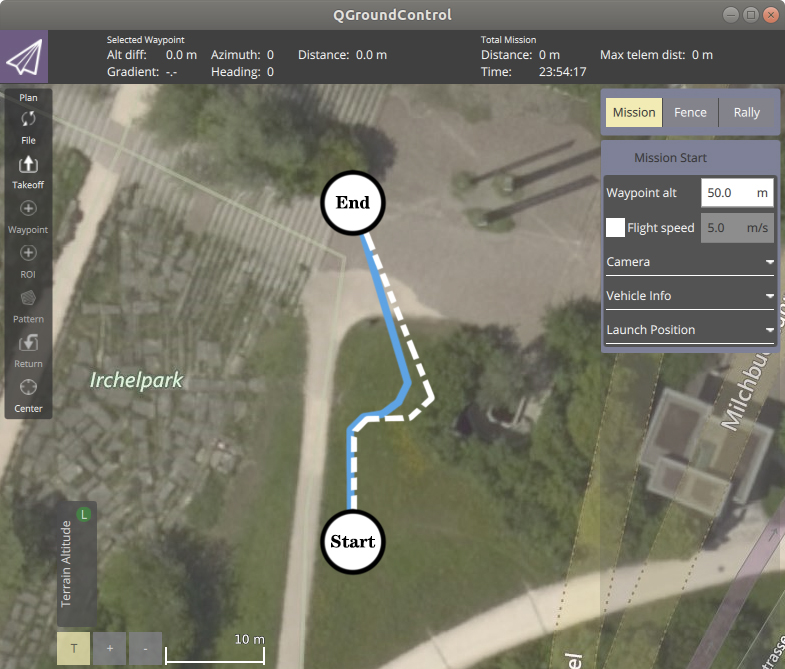
\includegraphics[width=0.95\linewidth]{oppositeFlightSimulation.jpg} 
	\caption{One flight simulation for the opposite flight experiment. Blue line: MCVI flight path; white line: simple flight path}
	\label{fig:oppositeFlightSimulation}
\end{figure}

\begin{table}[t]
	\caption{Opposite flight results; in bold, the best results}
	\label{tab:oppositeFlightResults}
	\centering
	\begin{tabular}{c|c|c}
		& rule-based & MCVI-based\\
		\hline 
		actNum & \textbf{4} & 5\\
		minDis & 2.51 & \textbf{2.95} \\
		maxDvtDis & 9.69 & \textbf{5.88} \\
		incFltDis & 14.83 & \textbf{9.67}\\
	\end{tabular}
\end{table}

In the first simulated experiment, we assume that the intruder aircraft starts from the destination of our own aircraft (viz. 30 meters North of the starting place of own aircraft) and flies straight towards the starting place of our own aircraft.
The flight paths of the mission while avoiding a collision are shown in Fig.~\ref{fig:oppositeFlightSimulation} and the average experimental results are summarized in Table~\ref{tab:oppositeFlightResults}.

Based on the \jMAVSim{} simulation, depicted in Fig.~\ref{fig:oppositeFlightSimulation}, we can see the flight path of own aircraft in the simulated map, where the blue solid line represents the flight path induced by the MCVI method while the white dashed line tracks the flight path given by the simple rule-based method. 
It can be intuitively seen from the figure that the MCVI method can reduce the useless avoidance distance of our own aircraft, and avoid the collision risk more effectively.

Table~\ref{tab:oppositeFlightResults} gives more details about the flight paths: 
we note that although the logic generated by MCVI based on the POMDP model takes 5 actions instead of 4 to reach the destination while avoiding the intruder aircraft, it does not results in an increase of the flight distance.
On the contrary, as shown in Fig.~\ref{fig:oppositeFlightSimulation} by the MCVI method's blue solid line being closer to the straight line between the terminal points than the simple method's white dashed line, the flight distance is increased by just 9.67 meters, about 5 meters less than the 14.83 meters of the simple method.
Furthermore, the MCVI-based approach increases the minimum distance (2.95 vs. 2.51 meters) from the intruder aircraft while deviating less (5.88 vs. 9.69 meters) from the optimal path without intruders than the simple method; 
this guarantees a higher safety level while decreasing the maximum deviation distance from the new flight path to the original mission flight path. 


\subsection{Simulated Intruder's Random Interfering Flight Experiment}
\label{ssec:randomInterferingFlight}

In the second simulated experiment, we assume that the intruder aircraft takes off from the midway between the start place and destination of our own aircraft (viz. 15 meters North of the starting place of our own aircraft). 
This time the intruder aircraft chooses randomly an action between bank-left, go-forward and bank-right, i.e., each one with probability $\frac{1}{3}$. 
Since the flight behavior of the intruder aircraft in this experiment is randomized, we repeated the simulation 50 times and then considered the average outcomes of the two scenarios against the same intruder's random choices, which can be reproduced by fixing the same random seed for the two scenarios. 

\begin{table}[t]
	\caption{Random interfering flight results; in bold, the best results}
	\label{tab:randomInterferingFlightAverageResults}
	\centering
	\begin{tabular}{c|cc|cc}
	& \multicolumn{2}{c|}{average value} & \multicolumn{2}{c}{median value}\\
	& rule-based & MCVI-based & rule-based & MCVI-based\\
	\hline
	actNum & \textbf{3.82} & 4.96 & \textbf{2.5} & 4 \\
	minDis & 5.54 & \textbf{6.06} & 5.88 & \textbf{6.04} \\
	maxDvtDis & 8.85 & \textbf{5.40} & 7.50 & \textbf{5.60} \\
	incFltDis & 9.14 & \textbf{7.10} & \textbf{6.67} & 6.87
	\end{tabular}
\end{table}
The statistics for this experiment are presented in Table~\ref{tab:randomInterferingFlightAverageResults};
as we can see, we have a behavior similar to the opposite flight experiment: 
although the logic generated by MCVI on the POMDP model banks on average one time more to avoid the intruder than the simple rule-based method, it is able to reduce the increased flight distance.
Furthermore, it increases the minimum distance between the two aircraft, which implies that the MCVI method gives a higher safety level when dealing with the random behavior of the intruder aircraft.
It is particularly noteworthy that when compared with the simple rule-based method, MCVI-based collision avoidance is able to save about $40\%$ of the maximum deviation distance between the actual flight path and the original mission flight path, which is a straight line between the designed takeoff and landing coordinates. 

We now give some more details about the safety level achieved by the two collision avoidance scenarios introduced in Section~\ref{ssec:experimentsConfiguration}.
Out of the 50 simulations for each of the two scenarios, 
both scenarios ensure that there is no collision since in none of the simulations the minimum distance was below $2$ meters, the value we set for NMAC;
the minimum distance has been at least $2.5$ meters.
There have been few simulations where the distance was about 3 meters and the majority above 4 meters, with the MCVI-based scenario usually keeping a larger distance.
This is reflected also by the average \emph{minDis} values reported in Table~\ref{tab:randomInterferingFlightAverageResults}, where the rule-based \emph{minDis} value is lower than the one for MCVI, which means that the former control policy got closer to the intruder than the latter one.

From these experiments, we obtain that the MCVI-based collision avoidance controller provides a better safety level, since it keeps a larger distance between our aircraft and the intruder than the rule-based controller.
This comes at the cost of banking the aircraft few more times, which still allows for reducing the increased flown distance.
The flown distance is also an aspect to be considered for drones and other unmanned aircraft, since the increased flight distance reduces the actual operative range of the aircraft, given the limited amount of energy stored in the batteries that can be used to power the aircraft.

While the experiments give a good indication about the safety level provided by the MCVI-based collision avoidance controller, there is no guarantee that it always avoids collisions.
We leave the formal analysis of its safety as future work.


\subsection{Actual Pixhawk Drone Flight Experiment}
\label{ssec:realDrone}

In the third experiment, we have taken the PX4 MCVI-based collision avoidance module we developed and uploaded it on a real Pixhawk drone we assembled ourselves. %, shown in Fig.~\ref{fig:RealDrone}. 
The flight mission is the same as for the previous experiments. 
The Pixhawk drone communicates to its ground station several data about the position and flight attitude.
Since the Pixhawk drone has no sensors for detecting intruders, we used the ground station to inject in the drone's PX4 control system the synthetic intruder from the opposite flight experiment presented in Section~\ref{ssec:oppositeFlight}.
We show in Fig.~\ref{fig:realFlightPath} the actual flight path flown by our drone as registered by the ground control station and superimposed on the map.

\begin{figure}[t]
	\centering 
	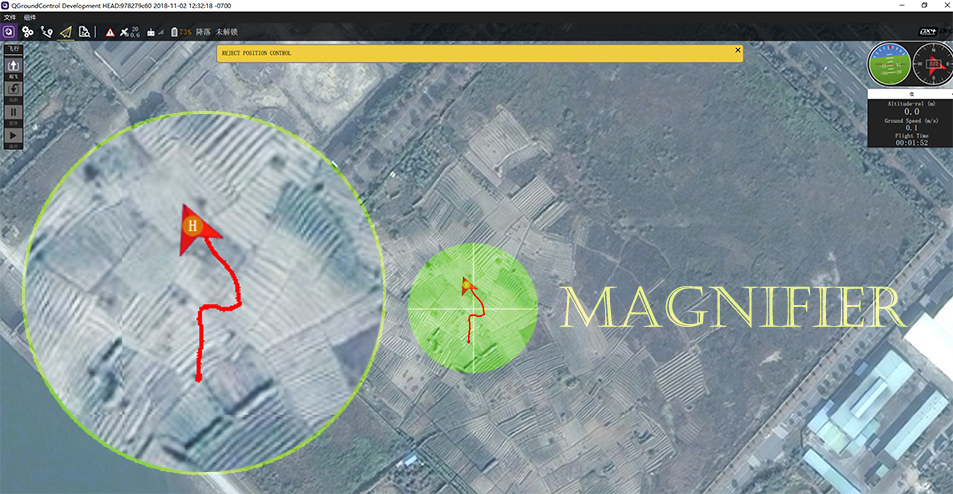
\includegraphics[width=1\linewidth]{realFlightPath.jpg}
	\caption{The actual Pixhawk drone flight path registered by the ground control station}
	\label{fig:realFlightPath}
\end{figure}

As we can see, the MCVI-based collision avoidance module works well not only in a synthetic environment, but also in the real world.
This suggests that the policy synthesis for specifically crafted POMDPs can improve the safety of unmanned aircraft equipped with a collision avoidance module basing its decisions on the synthesized policy.



\section{Conclusion}
\label{sec:conclusion}

We have constructed a collision avoidance system working with limited information, which also tried to save flying resources by means of reducing the change of the original flight path.
Our approach used a POMDP to model the collision avoidance system with only the destination information of our own aircraft and rough direction information of the intruder and then generated the collision resolution logic that maximizes the expected sum of rewards of selected actions.
We have implemented the collision avoidance module and embedded it into the PX4 flight control platform that can control real unmanned aircraft systems.
The effectiveness of our system is witnessed by the experimental evaluation in both a simulated environment and a real world scenario using a Pixhawk drone.

As future work, we consider to study the scalability of the MCVI approach to more detailed flight scenarios, such as the ones with the 3D environment, different aircraft speeds, more accurate observations given by better sensors, and so on.
Also, we plan to apply machine learning algorithms to improve the efficiency of the algorithm for searching an optimal policy.
Moreover, we also consider the use of rigorous methods, such as model checking, to ensure the correctness of the collision avoidance system.


\paragraph*{Acknowledgments.}
The authors are very thankful to Xuechao Sun and Junwen Li for helpful discussion and the assembly of the Pixhawk drone. 
This work has been supported by 
the Guangdong Science and Technology Department (grant no.\ 2018B010107004),
the Natural Science Foundation of Guangdong Province (grant no. 2019A1515011689), and 
the National Natural Science Foundation of China (grant nos.\ 61761136011, 61532019, 61836005).




\begin{thebibliography}{10}
\providecommand{\url}[1]{\texttt{#1}}
\providecommand{\urlprefix}{URL }
\providecommand{\doi}[1]{https://doi.org/#1}

\bibitem{DBLP:conf/rss/Bai-RSS-11}
Bai, H., Hsu, D., Kochenderfer, M.J., Lee, W.S.: Unmanned aircraft collision
  avoidance using continuous-state {POMDPs}. In: Durrant{-}Whyte, H.F., Roy,
  N., Abbeel, P. (eds.) Robotics: Science and Systems VII, University of
  Southern California, Los Angeles, CA, USA, June 27-30, 2011 (2011).
  \doi{10.15607/RSS.2011.VII.001},
  \url{http://www.roboticsproceedings.org/rss07/p01.html}

\bibitem{MCVI}
Bai, H., Hsu, D., Lee, W., Vien, N.: {Monte Carlo} value iteration for
  continuous-state {POMDPs}. Algorithmic Foundations of Robotics IX
  \textbf{68},  175--191 (2010). \doi{10.1007/978-3-642-17452-0\_11}

\bibitem{article2}
Hauskrecht, M.: Value-function approximations for partially observable {Markov}
  decision processes. Journal of Artificial Intelligence Research  \textbf{13},
   33--94 (2000). \doi{10.1613/jair.678}

\bibitem{article3}
Hazeghi, K., Puterman, M.: {Markov} decision processes: Discrete stochastic
  dynamic programming. Journal of the American Statistical Association
  \textbf{90}, ~392 (1995). \doi{10.2307/2291177}

\bibitem{Julian-2016}
Julian, K.D., Lopez, J., Brush, J.S., Owen, M.P., Kochenderfer, M.J.: Policy
  compression for aircraft collision avoidance systems. In: 2016 IEEE/AIAA 35th
  Digital Avionics Systems Conference (DASC). pp. 1--10 (2016)

\bibitem{article1}
Kaelbling, L., Littman, M., Cassandra, A.: Planning and acting in partially
  observable stochastic domains. Artificial Intelligence  \textbf{101},
  99--134 (1998). \doi{10.1016/S0004-3702(98)00023-X}

\bibitem{book}
Kamen, E.W., Su, J.K.: Introduction to Optimal Estimation (1999).
  \doi{10.1007/978-1-4471-0417-9\_3}

\bibitem{ACASX}
Kochenderfer, M., Chryssanthacopoulos, J.: Robust airborne collision avoidance
  through dynamic programming (2011)

\bibitem{article}
Kochenderfer, M., Holland, J., Chryssanthacopoulos, J.: Next generation
  airborne collision avoidance system. Lincoln Laboratory Journal  \textbf{19},
   17--33 (2012)

\bibitem{TCAS}
Kuchar, J., Drumm, A.: The traffic alert and collision avoidance system.
  Lincoln Laboratory Journal  \textbf{16}(2),  277--296 (2007)

\bibitem{sarsop}
Kurniawati, H., Hsu, D., Lee, W.S.: {SARSOP:} efficient point-based {POMDP}
  planning by approximating optimally reachable belief spaces. In: Robotics:
  Science and Systems IV (2008)

\bibitem{inproceedings}
Manfredi, G., Jestin, Y.: An introduction to {ACAS Xu} and the challenges
  ahead. In: DASC. pp.~1--9 (2016). \doi{10.1109/DASC.2016.7778055}

\bibitem{PBVI}
Pineau, J., Gordon, G., Thrun, S.: Point-based value iteration: An anytime
  algorithm for {POMDPs}. In: IJCAI. pp. 1025--1032 (2003)

\bibitem{pbvic}
Porta, J., Vlassis, N., Spaan, M., Poupart, P.: Point-based value iteration for
  continuous {POMDPs}. Journal of Machine Learning Research  \textbf{7},
  2329--2367 (2006)

\bibitem{Puterman05}
Puterman, M.L.: {Markov} Decision Processes: Discrete Stochastic Dynamic
  Programming. No.~594 in Wiley Series in Probability and Statistics, John
  Wiley \& Sons, Inc. (2005)

\bibitem{ASurveyofPBPOMDP}
Shani, G., Pineau, J., Kaplow, R.: A survey of point-based {POMDP} solvers.
  Auton Agent Multi-Agent Syst  \textbf{27},  1--51 (2013).
  \doi{10.1007/s10458-012-9200-2}

\bibitem{PBVII}
Smith, T., Simmons, R.: Point-based {POMDP} algorithms: Improved analysis and
  implementation. In: UAI. pp. 542--549 (2005)

\bibitem{Sondik78}
Sondik, E.J.: The optimal control of partially observable {Markov} processes
  over the infinite horizon: Discounted costs. Oper. Res.  \textbf{26}(2),
  282--304 (1978). \doi{10.1287/opre.26.2.282},
  \url{https://doi.org/10.1287/opre.26.2.282}

\bibitem{RLIntro}
Sutton, R.S., Barto, A.G.: Reinforcement learning - an introduction. Adaptive
  computation and machine learning, {MIT} Press (1998),
  \url{http://www.worldcat.org/oclc/37293240}

\bibitem{25}
Temizer, S., Kochenderfer, M., Kaelbling, L., Lozano-Perez, T., Kuchar, J.:
  Collision avoidance for unmanned aircraft using {Markov} decision processes.
  In: AIAA Guidance, Navigation, and Control Conference (2010).
  \doi{10.2514/6.2010-8040}

\bibitem{mcpomdp}
Thrun, S.: {Monte Carlo} {POMDPs}. In: NIPS. pp. 1064--1070 (1999)

\end{thebibliography}

\end{document}

